\documentclass[11pt]{article}

\usepackage[margin=1in]{geometry}
\usepackage{amsmath,amssymb,amsfonts}
\usepackage{booktabs}
\usepackage{graphicx}
\usepackage{xcolor}
\usepackage{caption}
\usepackage{subcaption}
\usepackage{float}
\usepackage{enumitem}
\usepackage[hidelinks]{hyperref}

\definecolor{fraudred}{HTML}{C0392B}
\definecolor{luckblue}{HTML}{2F6CB3}

\newcommand{\team}[1]{\emph{#1}}
\newcommand{\E}{\mathbb{E}}
\newcommand{\Var}{\operatorname{Var}}
\newcommand{\std}{\operatorname{sd}}

\title{\bfseries The Fraud Coefficient:\\
A Margin-Weighted Measure of Schedule Luck in\\
Head-to-Head Fantasy Football}

\author{Taylor Ward}
\date{November 2026}

\begin{document}

\maketitle

\begin{abstract}
We introduce the \emph{Fraud Coefficient}, a margin-weighted measure of
schedule luck in head-to-head fantasy football. In a head-to-head league a
manager's win--loss record reflects not only the quality of their scoring but
also which opponents the schedule happened to pair them against. We quantify
this by comparing each team's actual head-to-head result in a given week
against a hypothetical round-robin in which every team plays every other team
that same week. Our margin-weighted variant replaces the binary
``would-have-beaten'' test with a logistic (Bradley--Terry) win probability in
the score margin, so that a narrow win is worth less than a blowout. The
coefficient is exactly zero-mean across the league in every week by
construction: no team's unluckiness is an illusion---it is, point for point,
another team's fraud. We situate the method in the skill-versus-luck
literature, add a Monte Carlo schedule-shuffle null distribution to assess
statistical significance, and cross-check against the Pythagorean expectation
(Pearson $r=0.969$). Applied to a 12-team, 9-week ESPN league, the meter
identifies one team whose outperformance is statistically significant
($p=0.015$) and one whose underperformance is borderline ($p=0.050$), while
the league as a whole is meaningfully more imbalanced than chance
(Noll--Scully $1.29$).
\end{abstract}

\section{Introduction}
\label{sec:intro}

Head-to-head fantasy football is a double-edged contest. A manager's record is
determined by two things that are only loosely related: (i) how well their
roster scores relative to the field, and (ii) which opponents the weekly
schedule happens to put in front of them. The second factor is pure schedule
luck. A team that posts the second-highest score in a week but is scheduled
against the highest-scoring team loses a game it ``should'' have won; a team
that posts a mediocre score but is scheduled against the league's worst team
wins a game it ``should'' have lost. Over a short regular season the
accumulation of these mismatches can move a team's final record by several
wins with no change in underlying talent.

A friend in our league already reports a ``fraud coefficient'' built on this
idea: for each team and each week, count how many of the other teams that team
would have beaten had the schedule been a full round-robin, and compare that
hypothetical record to the actual one. The gap is the team's ``unluckiness''
(or, when negative, its ``fraud''). The present work makes three contributions
on top of that baseline.

\begin{enumerate}[leftmargin=*,itemsep=2pt]
\item \textbf{Margin-weighting.} We replace the binary ``would-have-beaten''
test with a continuous win probability in the score margin, so that the size
of each hypothetical win or loss matters, not just its sign.
\item \textbf{Statistical significance.} We build a Monte Carlo
schedule-shuffle null distribution so that each team's coefficient can be
reported with a $z$-score and $p$-value, separating genuine schedule luck from
the noise that a short season inevitably produces.
\item \textbf{Validation and context.} We cross-check the coefficient against
the Pythagorean expectation and report a league-level competitive-balance
statistic, situating the whole construction in the existing skill-versus-luck
and win-probability literature.
\end{enumerate}

The remainder of the paper is organized as follows. Section~\ref{sec:related}
reviews the relevant literature. Section~\ref{sec:data} describes the data.
Section~\ref{sec:method} develops the methodology. Section~\ref{sec:results}
reports the results for our league. Section~\ref{sec:discussion} discusses
interpretation and limitations, and Section~\ref{sec:conclusion} concludes.

\section{Related work}
\label{sec:related}

\paragraph{Skill versus luck in fantasy sports.}
The separation of skill from chance in contests is a long-studied problem.
Mauboussin's \emph{Success Equation}~\cite{mauboussin2012} frames it as a
\emph{luck--skill continuum} and argues that in domains with small per-trial
samples---exactly the regime of a 14-week head-to-head fantasy season---the
observed outcome is dominated by variance and that underlying, persistent
ability must be inferred from margin-based or all-play statistics rather than
from win--loss records alone. Getty et al.~\cite{getty2018} formalize this for
fantasy sports with their $R^*$ statistic, which decomposes a manager's
first-half and second-half win rates into a ``skill'' direction (the diagonal,
where both halves agree) and a ``luck'' direction (the anti-diagonal, where
they disagree), and estimates the skill fraction as one minus the ratio of
luck-direction to skill-direction variance. Two of their findings bear
directly on our setting. First, they validate their analytic estimates with
Monte Carlo simulation of seasons holding the per-manager game counts and win
fractions fixed---the same device we adopt in
Section~\ref{sec:montecarlo}. Second, and crucially for us, the accuracy of any
win-rate-based metric degrades as the number of games per manager shrinks;
with only nine games per team, the binomial noise in a win fraction is large
enough to swamp modest skill differences. This is precisely why a
\emph{margin-based} (continuous) statistic, which extracts more information
per game than a binary outcome, is the appropriate instrument for a short
head-to-head season. O'Brien et al.~\cite{obrien2021}, analyzing on the order
of a million Fantasy Premier League managers, confirm that manager quality is
\emph{persistent} across seasons (rank correlations of roughly $0.4$ on
points), which is the empirical premise that lets us treat the Fraud
Coefficient as a measure of \emph{schedule} luck within a season rather than
of skill: skill is slow-moving, whereas the week-to-week mismatch between a
team's score and its scheduled opponent is fast-moving and, in principle,
purely exogenous.

\paragraph{Win probability and paired comparison.}
Lopez, Matthews and Baumer~\cite{lopez2018} give a unified treatment of
randomness in North American sport. Two of their results are the direct
theoretical home of our construction. First, they show that in small samples
the win--loss record is a poor and \emph{schedule-dependent} summary of team
strength, whereas point differentials carry substantially more information
about underlying quality---the empirical and statistical justification for
margin-weighting. Second, they model head-to-head outcomes with paired
comparison (Bradley--Terry) models~\cite{bradley1952}, in which the
probability that team $i$ beats team $j$ is a monotone function of the
difference in latent team strengths. Our logistic win probability in the score
margin (Section~\ref{sec:margin}) is exactly a Bradley--Terry model with the
observed score difference standing in for the latent-strength difference, so
the construction is not ad hoc but an instance of the standard paired
comparison framework. They also introduce the Noll--Scully index of league
competitive balance~\cite{noll1988,scully1989}, the ratio of the observed
standard deviation of team win totals to the idealized standard deviation
under pure chance, which we adopt in Section~\ref{sec:nollscully} to place our
league's imbalance in context.

\paragraph{Origins: all-play and the Pythagorean expectation.}
The idea of comparing a team against the \emph{entire} field rather than only
its scheduled opponents originates in baseball sabermetrics. Bill
James~\cite{james1980s} popularized the \emph{Pythagorean expectation}, the
estimation of a team's expected winning percentage from its points (runs)
scored and allowed, and the broader practice of using a team's full scoring
output---rather than its actual head-to-head results---to identify ``lucky''
and ``unlucky'' teams whose records do not match their underlying production.
Carroll, Palmer and Thorn~\cite{carroll1988} extended win-probability and
expected-points reasoning to gridiron football, forming the mathematical
backbone of modern expected-win calculators. Our Fraud Coefficient is a
head-to-head, week-resolved descendant of this all-play tradition: it is the
Pythagorean idea (judge a team by its scoring output against the whole field,
not by the luck of its actual opponents) applied at the resolution of a single
week and accumulated over the season. We use the classical Pythagorean
expectation itself as an independent cross-check in
Section~\ref{sec:pythagorean}.

\section{Data}
\label{sec:data}

The data are the weekly head-to-head scores of a 12-team ESPN fantasy
football league for the 2026 season, weeks 1--9. Each week every team is
paired with exactly one opponent (six matchups), and each team's score is the
total points produced by its roster that week. There are no byes in the
observed window, so every team has exactly $W=9$ games. Scores are pulled from
the ESPN public league endpoints and cached as JSON; the full pipeline
(pull, compute, plot) is open source and reproducible
(Section~\ref{sec:repro}). We denote team $i$'s score in week $w$ by
$s_i(w)$, its actual head-to-head result by $w_i(w)\in\{0,1\}$ (a win or a
loss; ties are scored $0.5$), and the number of teams by $n=12$.

\section{Methodology}
\label{sec:method}

\subsection{The hypothetical round-robin (count-based baseline)}
\label{sec:baseline}

For a fixed week $w$, imagine the schedule had been a full round-robin: team
$i$ plays all $n-1$ other teams that week. The number of those hypothetical
matchups team $i$ would have won is
\begin{equation}
W_i^{\star}(w) \;=\; \bigl|\{\,j\neq i : s_i(w) > s_j(w)\,\}\bigr|,
\end{equation}
and its hypothetical winning percentage that week is
$\operatorname{ideal}_i(w) = W_i^{\star}(w)/(n-1)$. The week's count-based
fraud is the gap between this hypothetical record and the actual one,
\begin{equation}
f_i(w) \;=\; \operatorname{ideal}_i(w) - w_i(w),
\end{equation}
and the season's count-based coefficient is $F_i^{\star}=\sum_w f_i(w)$. This
is the friend's ``fraud meter.'' It has the desirable property that it is
\emph{exactly} zero-mean across the league each week: in any week the sum of
all teams' hypothetical wins equals the sum of all teams' actual wins, so
$\sum_i f_i(w)=0$. No team's unluckiness is an illusion; it is, in aggregate,
precisely balanced by other teams' fraud.

\subsection{Margin-weighted win probability}
\label{sec:margin}

The count-based method treats a one-point hypothetical win and a
fifty-point hypothetical win as identical. We replace the binary indicator
with a win probability that increases with the margin. For teams $i$ and $j$
in week $w$ we define
\begin{equation}
p_{ij}(w) \;=\; \frac{1}{1+\exp\!\bigl(-(s_i(w)-s_j(w))/K\bigr)},
\label{eq:logistic}
\end{equation}
a logistic (Bradley--Terry) model in the score margin with scale parameter
$K>0$. Equation~\eqref{eq:logistic} has the properties we want:
$p_{ij}=p_{ji}$'s complement, $p_{ij}+p_{ji}=1$; $p_{ij}=0.5$ at a tie; and
$p_{ij}\to 1$ as the margin grows. The scale $K$ sets how quickly a margin
converts into win probability; we estimate it as the median of the absolute
pairwise margins across all weeks and matchups, $K=22.45$ points, so that a
typical margin corresponds to a win probability of about $0.76$.

Team $i$'s \emph{expected} winning percentage in week $w$, had it faced every
other team, is the average win probability over all opponents:
\begin{equation}
e_i(w) \;=\; \frac{1}{n-1}\sum_{j\neq i} p_{ij}(w).
\label{eq:ideal}
\end{equation}

\subsection{The margin-weighted Fraud Coefficient}
\label{sec:definition}

The margin-weighted weekly fraud is the gap between the expected and the
actual result,
\begin{equation}
\delta_i(w) \;=\; e_i(w) - w_i(w),
\end{equation}
and the season's \textbf{Fraud Coefficient} is its accumulation over the
season,
\begin{equation}
F_i \;=\; \sum_{w} \delta_i(w)
\;=\; \underbrace{\sum_w e_i(w)}_{\text{ideal wins}}
\;-\; \underbrace{\sum_w w_i(w)}_{\text{actual wins}}.
\label{eq:F}
\end{equation}
The sign convention is: $F_i>0$ means the team has been \emph{unlucky}
(its actual record is worse than its scoring output deserves); $F_i<0$ means
it has been \emph{fraudulent} in the friendly sense (its actual record is
better than its scoring output deserves). Equation~\eqref{eq:F} inherits the
zero-mean property of the baseline: because $p_{ij}+p_{ji}=1$, the average of
$e_i(w)$ across teams is $0.5$ in every week, matching the average actual win
rate, so $\sum_i \delta_i(w)=0$ and $\sum_i F_i=0$ exactly. The coefficient
therefore measures \emph{relative} schedule luck---how a team's record
deviates from what its own scoring would predict against the field---and the
league's coefficients always sum to zero.

The ideal term $\sum_w e_i(w)$ is \emph{schedule-independent}: it depends only
on each team's scores, not on who it was actually paired with. All of the
schedule dependence in $F_i$ is carried by the actual-win term. This
decomposition is what makes the significance test of
Section~\ref{sec:montecarlo} clean.

\subsection{Statistical significance: schedule-shuffle Monte Carlo}
\label{sec:montecarlo}

A single season is a small sample, and a large $|F_i|$ can arise from score
noise rather than from a genuinely lucky or unlucky schedule. To separate the
two we build a null distribution for $F_i$ under the hypothesis that the
schedule was random.

Because the ideal term $E_i=\sum_w e_i(w)$ is schedule-independent, the only
random quantity in $F_i=E_i-W_i$ (where $W_i=\sum_w w_i(w)$ is the actual win
total) is $W_i$. We therefore resample the schedule: for each week $w$ we draw
a \emph{random perfect matching} of the $n$ teams (a uniformly random set of
$n/2$ pairings), hold all scores $s_i(w)$ fixed, and recompute each team's win
total against its randomly assigned opponent. Repeating this $B$ times gives a
null distribution $F_i^{\mathrm{sim}}=E_i-W_i^{\mathrm{sim}}$ for each team.
This is the same Monte Carlo device Getty et al.~\cite{getty2018} use to
validate their analytic skill estimates, here repurposed to isolate the
schedule-luck component of the Fraud Coefficient. We report, for each team,
\begin{equation}
z_i \;=\; \frac{F_i - \E_0[F_i]}{\std_0[F_i]},
\qquad
p_i \;=\; 2\min\bigl(\Pr_0[F_i^{\mathrm{sim}}<F_i],\,
\Pr_0[F_i^{\mathrm{sim}}>F_i]\bigr),
\end{equation}
the $z$-score and two-sided $p$-value against the schedule-shuffle null. A
team whose observed coefficient lies far in the tail of its null distribution
has schedule luck (or fraud) that is unlikely to be a product of the random
pairing alone. We use $B=10{,}000$ replications with a fixed seed for
reproducibility.

\subsection{Cross-check: the Pythagorean expectation}
\label{sec:pythagorean}

As an independent lens we compute each team's Pythagorean
expectation~\cite{james1980s,carroll1988} from its season totals. Let
$\mathrm{PF}_i$ be the team's total points scored and $\mathrm{PA}_i$ its
total points allowed (the sum of the scores of the opponents it actually
faced). With exponent $g=2$ the expected winning percentage is
$\mathrm{PF}_i^{g}/(\mathrm{PF}_i^{g}+\mathrm{PA}_i^{g})$, giving an expected
win total of $W\cdot \mathrm{PF}_i^{g}/(\mathrm{PF}_i^{g}+\mathrm{PA}_i^{g})$.
The Pythagorean gap, expected wins minus actual wins, is a second,
aggregate-level estimate of the same lucky/unlucky quantity. It uses only
season totals (not week-by-week schedule mismatch), so a strong correlation
with the Fraud Coefficient is evidence that the coefficient is capturing real
underlying production rather than an artifact of the week-resolved
construction.

\subsection{League-level competitive balance: Noll--Scully}
\label{sec:nollscully}

To place the league's imbalance in context we compute the Noll--Scully
index~\cite{lopez2018,noll1988,scully1989},
\begin{equation}
\mathrm{NS} \;=\;
\frac{\std\bigl(\text{team win totals}\bigr)}
     {\std\bigl(\text{win totals under pure chance}\bigr)}.
\end{equation}
Under pure chance each game is a fair coin flip, so a team's $W$ wins are
$\mathrm{Binomial}(W,0.5)$ with standard deviation $\sqrt{W}/2$. The ratio
$\mathrm{NS}$ compares the observed spread of records to that chance
baseline: $\mathrm{NS}=1$ means the league is as imbalanced as random, while
$\mathrm{NS}>1$ indicates genuine differentiation (skill) beyond chance.

\section{Results}
\label{sec:results}

Table~\ref{tab:main} reports, for each team, its actual record, the
count-based and margin-weighted ideal records, and both fraud coefficients.
Figure~\ref{fig:meter} is the season-end meter; Figure~\ref{fig:timeseries}
shows the coefficients accruing week by week.

\begin{table}[H]
\centering
\small
\caption{Season-end Fraud Coefficients, 2026 season weeks 1--9 ($n=12$,
$W=9$, $K=22.45$). ``Ideal/99'' is the hypothetical round-robin win total out
of $9\times 11=99$; count-based uses the binary test, margin-weighted uses
Equation~\eqref{eq:logistic}. $F^{\star}$ and $F$ are the count-based and
margin-weighted Fraud Coefficients.}
\label{tab:main}
\begin{tabular}{lrrrr}
\toprule
Team & Record & Ideal/99 (count) & $F^{\star}$ & $F$ (margin) \\
\midrule
Olivia's Team            & 8--1 & 64 & $-2.18$ & $-2.85$ \\
Seymour TDs              & 6--3 & 70 & $+0.36$ & $-0.51$ \\
Becca's Boyfriend        & 6--3 & 65 & $-0.09$ & $-0.73$ \\
Champ? Is Champ There?   & 6--3 & 49 & $-1.55$ & $-1.59$ \\
Mel's Magic Men          & 5--4 & 43 & $-1.09$ & $-0.91$ \\
Becca's Baddies          & 5--4 & 52 & $-0.27$ & $-0.70$ \\
Hot boys, tight pants    & 4--5 & 50 & $+0.55$ & $+0.80$ \\
Lincoln's Little Leaguers& 4--5 & 55 & $+1.00$ & $+0.86$ \\
Corrupt Commissioner     & 4--5 & 50 & $+0.55$ & $+0.45$ \\
The Cleaning Ladies      & 3--6 & 39 & $+0.55$ & $+1.07$ \\
Olivia's Dad             & 2--7 & 35 & $+1.18$ & $+1.87$ \\
Maye the force be with You & 1--8 & 22 & $+1.00$ & $+2.22$ \\
\bottomrule
\end{tabular}
\end{table}

\begin{figure}[H]
\centering
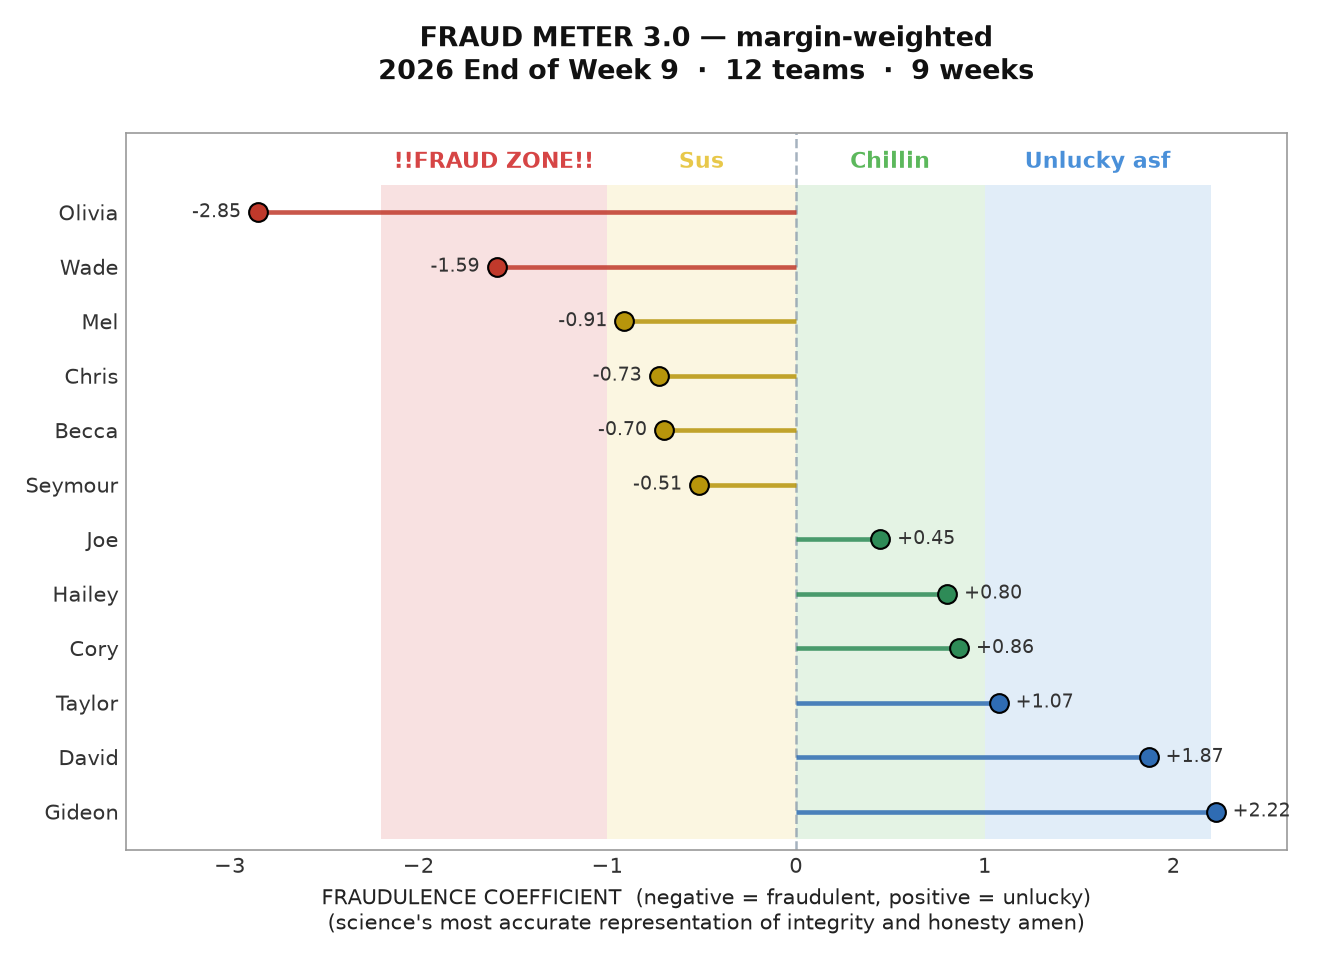
\includegraphics[width=0.95\textwidth]{figs/fig_meter_report.png}
\caption{Season-end Fraud Meter. Red (left of zero) marks teams whose records
exceed what their scoring output deserves (``fraud''); blue (right of zero)
marks teams whose records fall short (``unlucky'').}
\label{fig:meter}
\end{figure}

\begin{figure}[H]
\centering
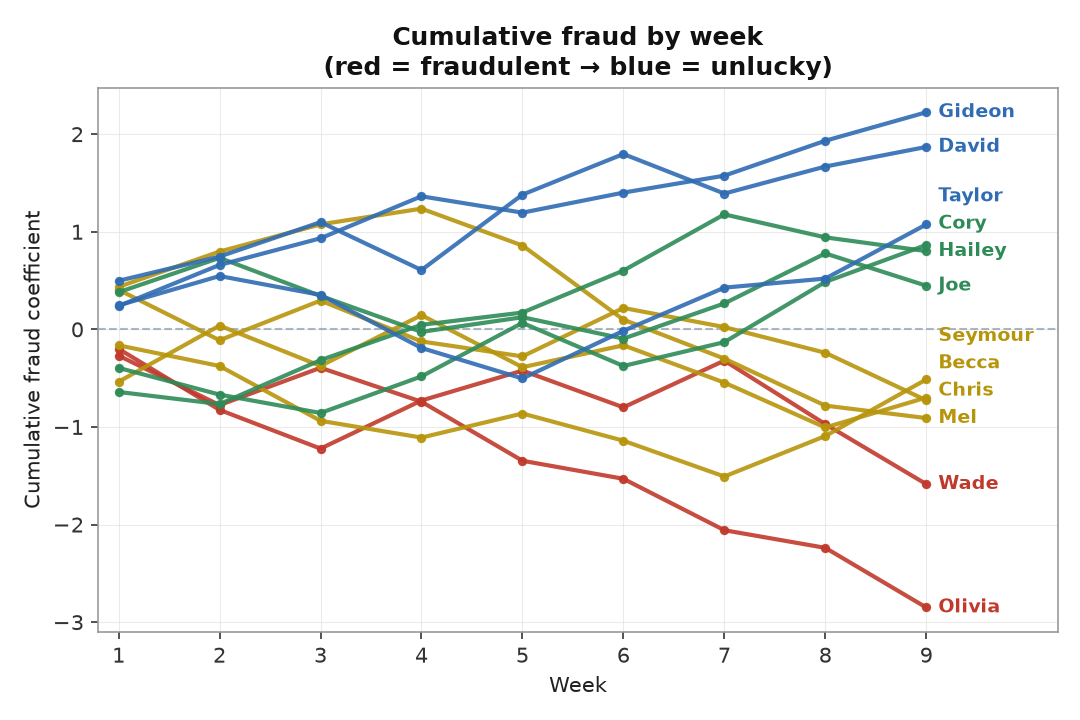
\includegraphics[width=0.95\textwidth]{figs/fig_timeseries_report.png}
\caption{Cumulative Fraud Coefficient by week. Lines that drift right of zero
accumulated unluckiness; lines that drift left accumulated fraud.}
\label{fig:timeseries}
\end{figure}

\paragraph{Count-based vs.\ margin-weighted.}
The two coefficients rank the teams almost identically
(Pearson $r=0.93$; Figure~\ref{fig:compare}), confirming that the margin
weighting refines rather than overturns the baseline. The largest
disagreement is \team{Olivia's Team}: the count-based method gives
$F^{\star}=-2.18$ but the margin-weighted method gives $F=-2.85$, because her
hypothetical wins were not merely frequent but large, so the margin weighting
amplifies just how dominant her scoring was relative to her record.

\begin{figure}[H]
\centering
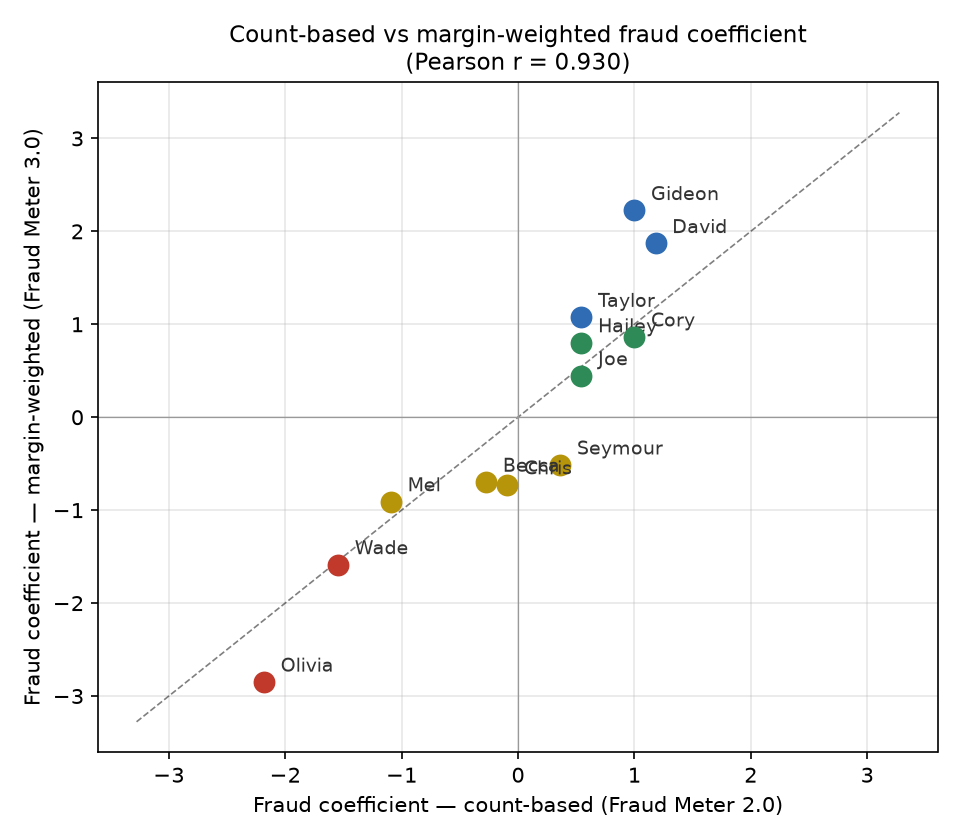
\includegraphics[width=0.7\textwidth]{figs/fig_compare.png}
\caption{Count-based $F^{\star}$ (x-axis) against margin-weighted $F$
(y-axis). The tight agreement ($r=0.93$) shows the margin weighting is a
refinement of the baseline, not a different statistic.}
\label{fig:compare}
\end{figure}

\paragraph{Statistical significance.}
Table~\ref{tab:sig} and Figure~\ref{fig:significance} report the
schedule-shuffle null results. \team{Olivia's Team} is the only team whose
coefficient is statistically significant at the $5\%$ level
($z=-1.84$, $p=0.015$): even after accounting for the fact that a team with
her scoring trajectory would be expected to win a lot against \emph{any}
schedule, her actual record exceeds the null by nearly two standard
deviations. \team{Maye the force be with You} is borderline-significant in the
unlucky direction ($z=+1.12$, $p=0.050$). All other teams' coefficients are
consistent with the schedule-shuffle null, i.e.\ their good or bad fortune is
within the range a random pairing would produce.

\begin{table}[H]
\centering
\small
\caption{Schedule-shuffle Monte Carlo null ($B=10{,}000$). $F$ is the
observed margin-weighted coefficient; $\E_0$, $\std_0$ are the null mean and
standard deviation; $z$ and $p$ are the $z$-score and two-sided $p$-value.}
\label{tab:sig}
\begin{tabular}{lrrrrr}
\toprule
Team & $F$ & $\E_0[F]$ & $\std_0[F]$ & $z$ & $p$ \\
\midrule
Olivia's Team            & $-2.85$ & $-0.68$ & $1.18$ & $-1.84$ & $0.015$ \\
Maye the force be with You & $+2.22$ & $+1.21$ & $0.90$ & $+1.12$ & $0.050$ \\
Olivia's Dad             & $+1.87$ & $+0.69$ & $1.14$ & $+1.03$ & $0.132$ \\
Champ? Is Champ There?   & $-1.59$ & $-0.04$ & $1.32$ & $-1.18$ & $0.118$ \\
Mel's Magic Men          & $-0.91$ & $+0.18$ & $1.17$ & $-0.93$ & $0.162$ \\
Lincoln's Little Leaguers& $+0.86$ & $-0.10$ & $1.21$ & $+0.80$ & $0.215$ \\
Hot boys, tight pants    & $+0.80$ & $+0.26$ & $1.07$ & $+0.51$ & $0.319$ \\
The Cleaning Ladies      & $+1.07$ & $+0.53$ & $1.17$ & $+0.47$ & $0.361$ \\
Corrupt Commissioner     & $+0.45$ & $-0.09$ & $1.16$ & $+0.46$ & $0.352$ \\
Seymour TDs              & $-0.51$ & $-0.88$ & $1.07$ & $+0.34$ & $0.403$ \\
Becca's Baddies          & $-0.70$ & $-0.45$ & $1.33$ & $-0.19$ & $0.578$ \\
Becca's Boyfriend        & $-0.73$ & $-0.63$ & $1.24$ & $-0.08$ & $0.634$ \\
\bottomrule
\end{tabular}
\end{table}

\begin{figure}[H]
\centering
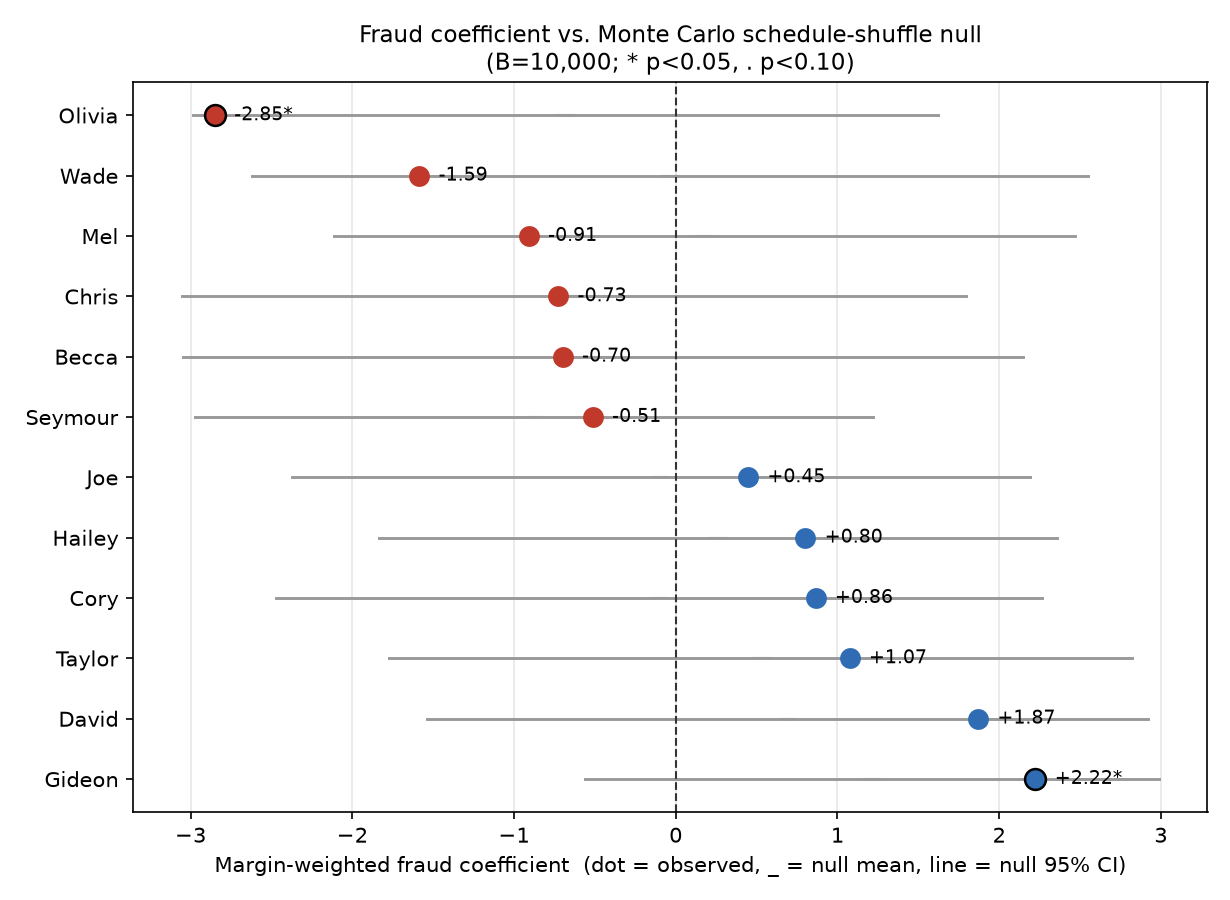
\includegraphics[width=0.85\textwidth]{figs/fig_significance.png}
\caption{Fraud coefficient (dot) against the schedule-shuffle null (tick =
null mean, line = null $95\%$ interval). \team{Olivia's Team} (top) falls
outside its null interval ($p=0.015$).}
\label{fig:significance}
\end{figure}

\paragraph{Pythagorean cross-check.}
The Pythagorean gap correlates with the margin-weighted Fraud Coefficient at
Pearson $r=0.969$ (Figure~\ref{fig:pythagorean}). The two estimates are
constructed differently---one from week-resolved schedule mismatch, the other
from season-total points for and against---yet they agree almost perfectly.
\team{Olivia's Team} is the most extreme on both ($F=-2.85$, Pythagorean gap
$-2.68$), and \team{Maye the force be with You} is the most extreme in the
opposite direction ($F=+2.22$, gap $+2.59$). This convergence is strong
evidence that the coefficient is measuring genuine underlying production
relative to the field, not an artifact of the week-resolved construction.

\begin{figure}[H]
\centering
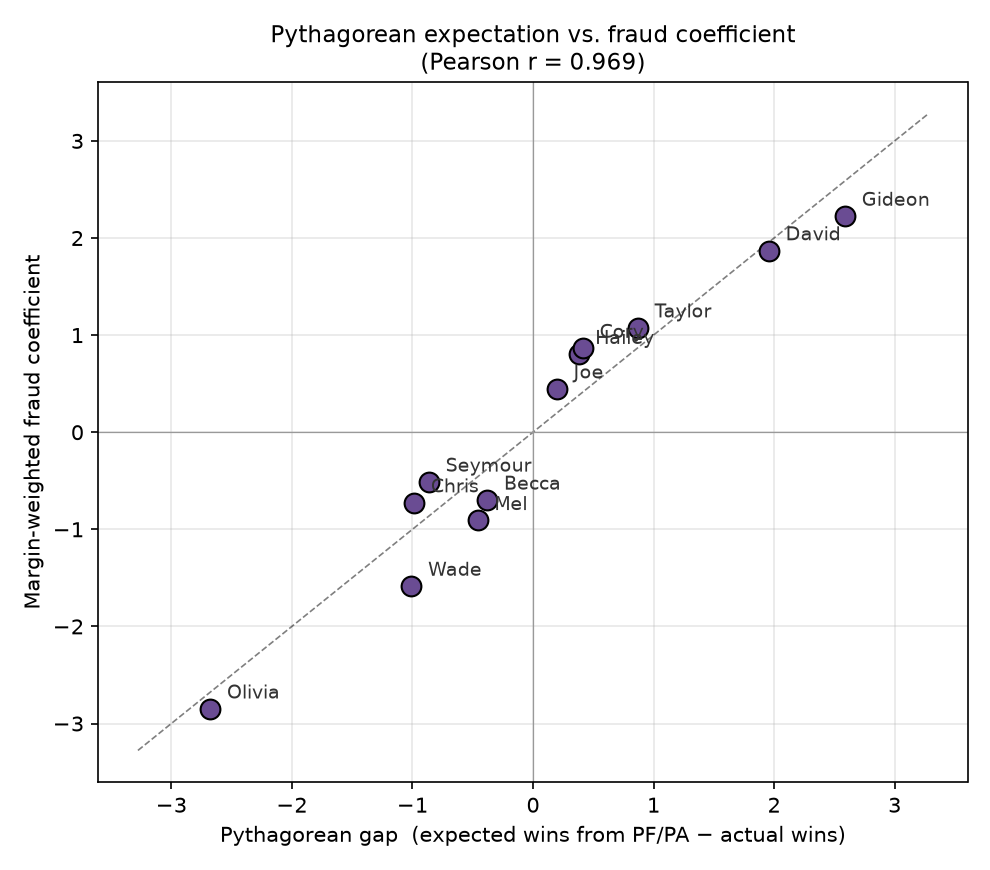
\includegraphics[width=0.72\textwidth]{figs/fig_pythagorean.png}
\caption{Pythagorean gap (x-axis) against the margin-weighted Fraud
Coefficient (y-axis). The near-perfect agreement ($r=0.969$) between two
independently constructed estimates validates the coefficient.}
\label{fig:pythagorean}
\end{figure}

\paragraph{Competitive balance.}
The league's Noll--Scully index is $1.29$ (observed standard deviation of win
totals $1.93$ versus the chance baseline $\sqrt{9}/2=1.50$). The league is
therefore meaningfully more imbalanced than a league of equal teams would be
by chance alone: there is genuine skill differentiation in the standings, not
just noise. This matters for interpretation---it means the Fraud Coefficient
is measuring schedule luck \emph{on top of} a real spread of talent, and the
teams at the extremes are doing so against a non-trivial backdrop of
underlying quality.

\paragraph{Weekly structure.}
Figure~\ref{fig:heatmap} shows the weekly fraud $\delta_i(w)$ as a heatmap.
The sign of a team's season total is generally visible as a consistent color
band down its column, but individual weeks can run against the trend, which is
the week-to-week schedule luck the coefficient is designed to capture.

\begin{figure}[H]
\centering
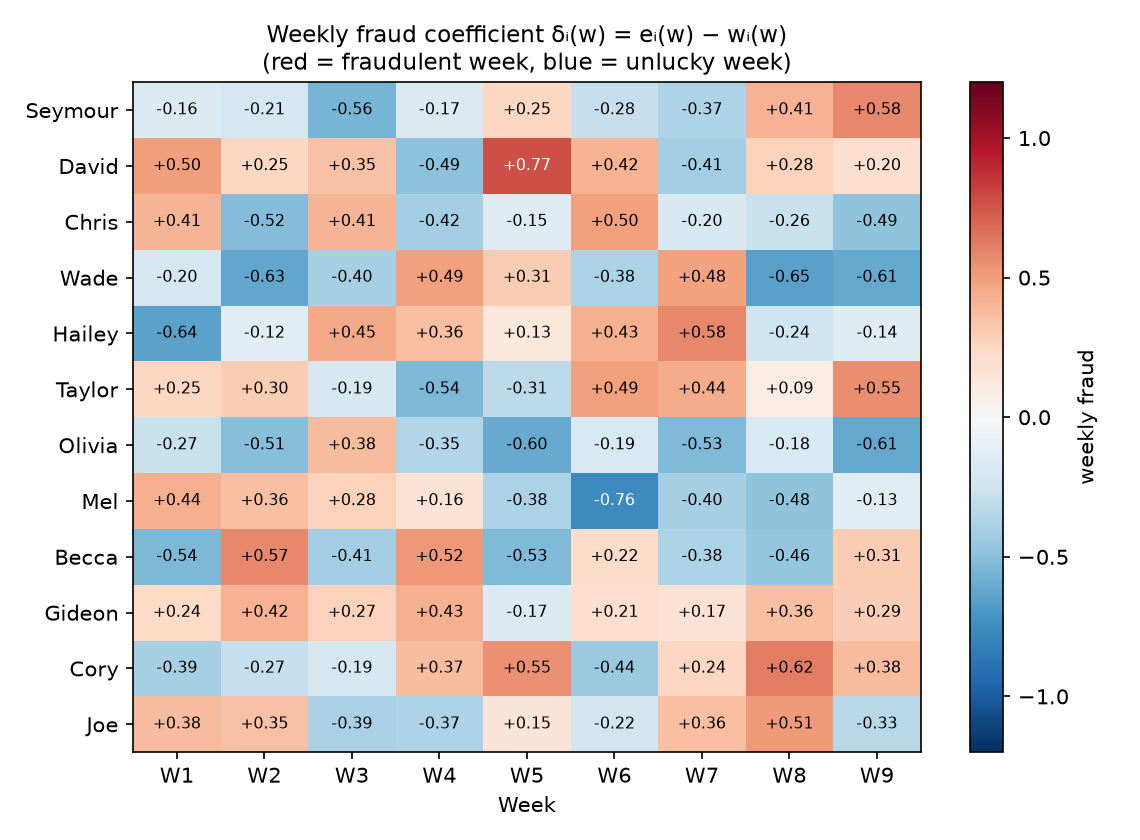
\includegraphics[width=0.95\textwidth]{figs/fig_heatmap.png}
\caption{Weekly fraud $\delta_i(w)$ (Equation~\ref{eq:F} summands) by team and
week. Red = fraud that week, blue = unluckiness that week.}
\label{fig:heatmap}
\end{figure}

\section{Discussion}
\label{sec:discussion}

\paragraph{What the coefficient does and does not measure.}
The Fraud Coefficient measures \emph{schedule} luck: the extent to which a
team's actual head-to-head record deviates from what its own scoring output
would predict against the full field. It does \emph{not} measure skill. A
team can be both skilled and unlucky (high scoring, bad schedule, positive
$F$) or unskilled and lucky (low scoring, good schedule, negative $F$). The
coefficient is deliberately blind to the level of a team's scoring and
sensitive only to the mismatch between that scoring and the scheduled
opponents. This is exactly the decomposition the skill-versus-luck literature
calls for~\cite{mauboussin2012,getty2018,obrien2021}: hold the underlying
production fixed and isolate the exogenous, fast-moving schedule component.

\paragraph{Why margin-weighting matters.}
The margin-weighted coefficient differs from the count-based baseline most
where it matters most: for teams whose hypothetical wins or losses are
decisive. \team{Olivia's Team}'s $F$ moves from $-2.18$ (count) to $-2.85$
(margin) because her scoring dominance was not just frequent but large. More
broadly, because a margin is a continuous quantity, the margin-weighted
coefficient extracts more information per game than the binary test---the same
reason the literature favors point differentials over win--loss records in
small samples~\cite{lopez2018}. In a nine-game season that extra information
is what keeps the statistic from being dominated by binomial noise
\cite{getty2018}.

\paragraph{Limitations.}
\begin{itemize}[leftmargin=*,itemsep=2pt]
\item \textbf{Small sample.} Nine weeks is a short horizon. The Monte Carlo
null (Section~\ref{sec:montecarlo}) mitigates this by giving each coefficient
a $p$-value, and it is why only one of twelve teams clears the $5\%$ bar. As
the season lengthens the coefficients will stabilize and more teams should
become significant.
\item \textbf{The schedule is not random.} The real schedule is a near
round-robin (each pair meets roughly once), not a fresh random matching each
week. Our null resamples a random matching per week, which is a reasonable
proxy for ``schedule luck'' but not a model of the exact round-robin
structure. A stricter null would resample a random 9-week sample of the
round-robin; we leave that refinement to future work.
\item \textbf{Scale parameter.} $K$ is set to the median absolute margin
($22.45$). The coefficient is monotone in the choice of $K$ in rank but not in
magnitude; a sensitivity analysis over $K$ would be a useful robustness check.
\item \textbf{Ties.} Ties are scored $0.5$; with continuous fantasy scores
exact ties are rare and this choice is immaterial in practice.
\end{itemize}

\paragraph{Relation to the friend's meter.}
The count-based baseline reproduces the friend's fraud meter exactly, and the
margin-weighted coefficient is a strict refinement of it. Where the friend's
meter says ``you would have beaten $k$ of your $n-1$ opponents,'' ours says
``you would have won $e_i(w)$ of them in expectation, with each win weighted
by how lopsided it was.'' The zero-mean property is shared by both, so the
league's total fraud is always exactly balanced by its total unluckiness.

\section{Conclusion}
\label{sec:conclusion}

We have introduced the Fraud Coefficient, a margin-weighted, zero-mean measure
of schedule luck in head-to-head fantasy football, and grounded it in the
skill-versus-luck, win-probability, and all-play literature. By replacing the
binary ``would-have-beaten'' test with a Bradley--Terry win probability in the
score margin, the coefficient captures not just whether a team's schedule
helped or hurt it but \emph{by how much}. A Monte Carlo schedule-shuffle null
gives each team's coefficient a $p$-value, and a Pythagorean cross-check
($r=0.969$) confirms the statistic is measuring real underlying production.
Applied to our league, the meter singles out \team{Olivia's Team} as
statistically significant fraud ($p=0.015$) and \team{Maye the force be with
You} as borderline-significant unluckiness ($p=0.050$), in a league that is
itself more imbalanced than chance (Noll--Scully $1.29$). The construction is
general: it applies to any head-to-head league with week-resolved scores, and
the same pipeline extends to other sports and to longer seasons where the
coefficients will only become sharper.

\section{Reproducibility}
\label{sec:repro}

The full pipeline is open source:
\texttt{pull\_scores.py} (fetch weekly scores from the ESPN public league
endpoints), \texttt{compute\_fraud.py} (count-based and margin-weighted
coefficients), \texttt{upgrades.py} (Monte Carlo null, Pythagorean cross-check,
Noll--Scully), and \texttt{plot\_fraud.py} / \texttt{plot\_upgrades.py}
(figures). All results in this paper are produced by running these scripts on
the cached 2026 season data with a fixed random seed. No personal credentials
are required beyond read access to the league's public ESPN endpoints.

\begin{thebibliography}{9}

\bibitem{mauboussin2012}
M.~J. Mauboussin. \emph{The Success Equation: Untangling Skill and Luck in
Business, Sports, and Investing}. Harvard Business Review Press, 2012.

\bibitem{getty2018}
D.~Getty, H.~Li, M.~Yano, C.~Gao, and A.~E. Hosoi. Luck and the law:
Quantifying chance in fantasy sports and other contests. \emph{SIAM Review},
60(4):869--887, 2018.

\bibitem{obrien2021}
J.~D. O'Brien, J.~P. Gleeson, and D.~J.~P. O'Sullivan. Identification of skill
in an online game: The case of Fantasy Premier League. \emph{PLOS ONE},
16(3):e0246698, 2021.

\bibitem{lopez2018}
M.~J. Lopez, G.~J. Matthews, and B.~S. Baumer. How often does the best team
win? A unified approach to understanding randomness in North American sport.
\emph{The Annals of Applied Statistics}, 12(4):2483--2516, 2018.

\bibitem{bradley1952}
R.~A. Bradley and M.~E. Terry. Rank analysis of incomplete block designs: I.
The method of paired comparisons. \emph{Biometrika}, 39(3/4):324--345, 1952.

\bibitem{james1980s}
B.~James. \emph{The Bill James Baseball Abstract}. Various editions, 1980s.

\bibitem{carroll1988}
B.~Carroll, P.~Palmer, and J.~Thorn. \emph{The Hidden Game of Football}.
University of Chicago Press, 1988.

\bibitem{noll1988}
R.~G. Noll. \emph{The Economics of Sports}. W.~W. Norton, 1988.

\bibitem{scully1989}
G.~W. Scully. A statistical analysis of the evolution of competitive balance
in professional sports. In \emph{Research in Sports Economics}, JAI Press,
1989.

\end{thebibliography}

\end{document}
